\section{Assessing the Performance Impact}

\label{sec:predictimprove}

%Fixing false sharing problems can be non-trivial, even with precise information about a particular false sharing problem. Several problems may occur. The first problem is that some false sharing problems can be insignificant. For example, \sheriff{} reports false sharing problems in word\_count or reverse\_index applications in Phoenix benchmark suites. However, fixing  them brings negligible performance benefit. The second problem is that fixing false sharing problem may even slow down the program because of excessive memory consumption or lose of locality, as observed by Zhao et. al. ~\cite{qinzhao}. 

To prove its concept, \cheetah{} currently predicts the performance impact for programs with simple fork-join models, shown as Figure~\ref{fig:forkjoinmodel}. 
The fork-join model is the most important and popular model in multithreading applications, as evidenced by all evaluated applications in this paper. 

\begin{figure*}[ht!]
\begin{center}
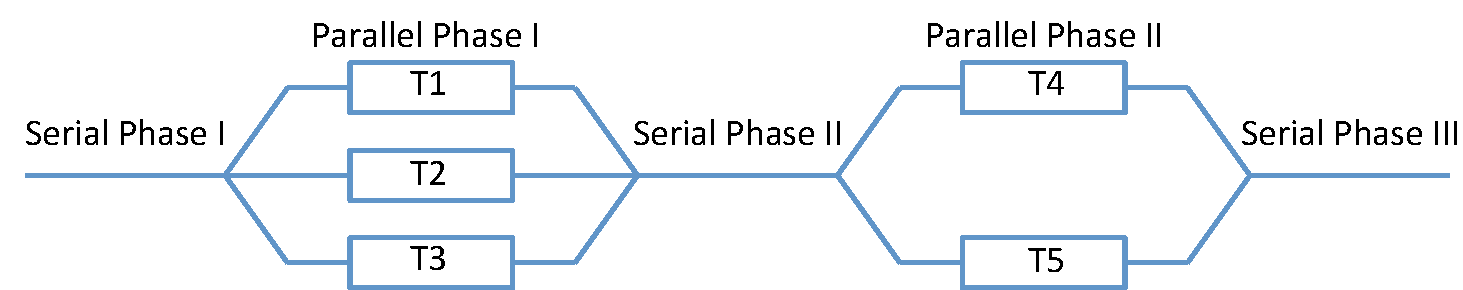
\includegraphics[width=6.5in]{figure/forkjoin}
\end{center}
\caption{Currently \Cheetah{} can predict the performance impact of false sharing inside applications with the normal fork-join model.
\label{fig:forkjoinmodel}}
\end{figure*}


%\cheetah{} collects the execution information on different phases, different threads, and different objects. 

This section will present the details of \cheetah{}'s prediction. Let's describe the general idea using the Figure~\ref{fig:forkjoinmodel} as an example. In this example, only thread $T1$ and $T2$ are involved in a falsely-shared object $O$, \cheetah{} has to know the following information:

\begin{itemize}
\item $Cycles\_O$: cycles of accesses on the object $O$.
\item $Accesses\_O$: the number of accesses on the object $O$.  
\item $Cycles\_{nofs}$: average cycles of every memory access on non-FS objects. 
\item The execution time of different threads.  
\item The execution time of different phases. 
\end{itemize}

After getting all information, \cheetah{} first computes the possible improvement rate by using $Cycles\_O$, $Accesses\_O$ and $Cycles\_{nofs}$ as EQ.(\ref{eq:improvement2}). 
\begin{equation}
\label{eq:improvement2}
 ImproveRate = (Accesses\_O * Cycles\_{nofs})/Cycles\_O;
\end{equation} 

Using the $ImproveRate$, we can compute the possible runtime of $T1$ and $T2$ after fixing the false sharing problem of object $O$, which are equal to the product of the actual runtime and $ImproveRate$. If the computed runtime is less than the length of $T3$ in parallel phase I, fixing the false sharing problem of object $O$ won't contribute any performance improvement of the program. Otherwise, it can benefit the performance. Then we compute the new runtime of parallel phase I, which equals to the longest runtime of thread $T1$, $T2$ or $T3$. Based on this, we computes the new runtime of this program, where the execution time of other phases should not be affected. In the end, \cheetah{} predicts the possible performance rate of fixing every false sharing problem so that programs can focus on those important problems. 

\subsection{Collecting Execution Information}
\label{sec:getactualtime}

\paragraph{Threads Model Information:} For fork-join models, only the main/initial thread can perform spawning operations. It is easy to verify this by intercepting spawning functions, such as the \texttt{pthread\_create} functions of programs using the \texttt{pthreads} library. 

\paragraph{Phase information:} \Cheetah{} collects the execution time of different serial and parallel phases using RDTSC (ReaD-Time Stamp Counter) on X86 machines.  The difference between the stopping point and the starting point will be considered as the length of a phase. It is relatively easy for \cheetah{} to collect the length of serial phases since \cheetah{} intercepts the spawning operations. For the same reason, \cheetah{} gets the timestamps of the starting point and the stopping point of each thread, then uses the longest span of each thread as the length of every parallel phase. \Cheetah{} also tracks the number of accesses and the cycles of every accesses in serial phases. It uses the average cycles of every memory access in serial phases to be the $Cycles\_{nofs}$ discussed above.  
 
\paragraph{Threads Information:} \Cheetah{} collects the following information of different threads: execution time, number of accesses, and number of cycles of all memory accesses. 

\paragraph{Objects Information:}
For each cache line, \cheetah{} gathers the number of cycles on each cache line. \cheetah{} also collect the number of accesses on each word. Thus, we can compute the number of cycles and accesses on falsely-shared objects. 
 
\subsection{Predicting Execution Time after Fixes}
\label{sec:predicttime}

\cheetah{} predicts the execution time after fixes by replacing the actual cycles of every memory access on a falsely-shared object with the average cycles of a memory access without false sharing. 

According to this, \cheetah{} should know the average cycles of a memory access without false sharing and true sharing. \Cheetah{} actually utilizes the cycles of every memory access in serial phases (denoted as $Cycles_{nofs}$) to approximate this value, which is reasonable since all memory accesses in serial phases should not involve in both false sharing and true sharing. 

Actual cycles of every memory access that are involving in a falsely-shared object can be changed from one execution to another. Thus, \cheetah{} utilizes the total number of all memory accesses instead to predict the performance impact. \Cheetah{} computes the possible performance improvement prediction in the following steps.
 
\begin{enumerate}
\item \cheetah{} first compute the total number of accesses ($Accesses_{fs}$) on suspected cache lines and the total cycles of accesses ($Cycles_{fs}$) on suspected cache lines.

\item For threads that are involved a particular false sharing, \cheetah{} then compute the total number of accesses ($Accesses_{threads}$) and the total cycle of accesses ($Cycles_{threads}$). 

\item \Cheetah{} computes the estimated cycles of those threads that are involved in false sharing according to the formula $Cycles_{pred} = Cycles_{threads} - Cycles_{fs} + Accesses_{fs} * AverageCycles_{nofs}$. 

\item  Based on this, \cheetah{} will compute the performance improvement on threads that are involved in false sharing.
$RT_{threads} = Cycles_{threads}  $. 

\end{enumerate}



\cheetah{} will utilize the latency information of every access to predict the performance impact of a certain false sharing instance. These latency information, normally CPU cycles of every sampled memory access, can be provided by hardware PMUs. \Cheetah{} plans to track detailed memory accesses on falsely-shared objects and on normal objects without false sharing. Thus, we can know the average cycles of every memory access without false sharing. 

\cheetah{} provides a upper bound on performance improvement after fixes. 

It is note that sampling based approaches can actually 
.

We only compute the cycles and threads for the parallel phases. 

\subsection{Predicting Performance Improvement}

%There are several steps to evaluate the performance impact. We will consider the average cycles on every access in serial phases as $Cycles_{serial}$. 

 % How to avoid huge performance overhead? We introducing per-thread recording mechanism. 

% How to actually predict the performance improvement? A thread may have the serial part and parallel part. We have to identify the serial part and parallel part. 

% How to handle different CPUs? For example, we may start 16 threads on 8 CPUs. 

% Can we get the resolute time on each phase? We are using this to calculate the performance improvement.  We also copy the whole memory accesses information out before transferring phases. 

% What if only two threads only accesses a specific cache line and other threads didn't accesses that? We can actually check the word level's accesses to find out those number of threads that are accesses this tid. We could also verify whether those memory accesses are on the critical path or not. 

% We should use actual tid instead of thread index to identify threads. 

% We should remove the write-invoked tracking since we have to check the number of accesses. Thus, we actually don't care those ones that are happened in the serial phase. Because we won't actual change its performance initially. 



% The total number of memory accesses on an addresses

% The total latency of accessing an address

% The total number of memory accesses for each thread. 

% The total latency of all memory accesses for each thread  

% All memory accesses of each thread

% All memory accesses in total = Sum of (memory accesses of each thread)

% Total latency of all memory accesses for each thread. 